\hypertarget{Predict_8h}{
\section{Predict.h File Reference}
\label{Predict_8h}\index{Predict.h@{Predict.h}}
}


This graph shows which files directly or indirectly include this file:\begin{figure}[H]
\begin{center}
\leavevmode
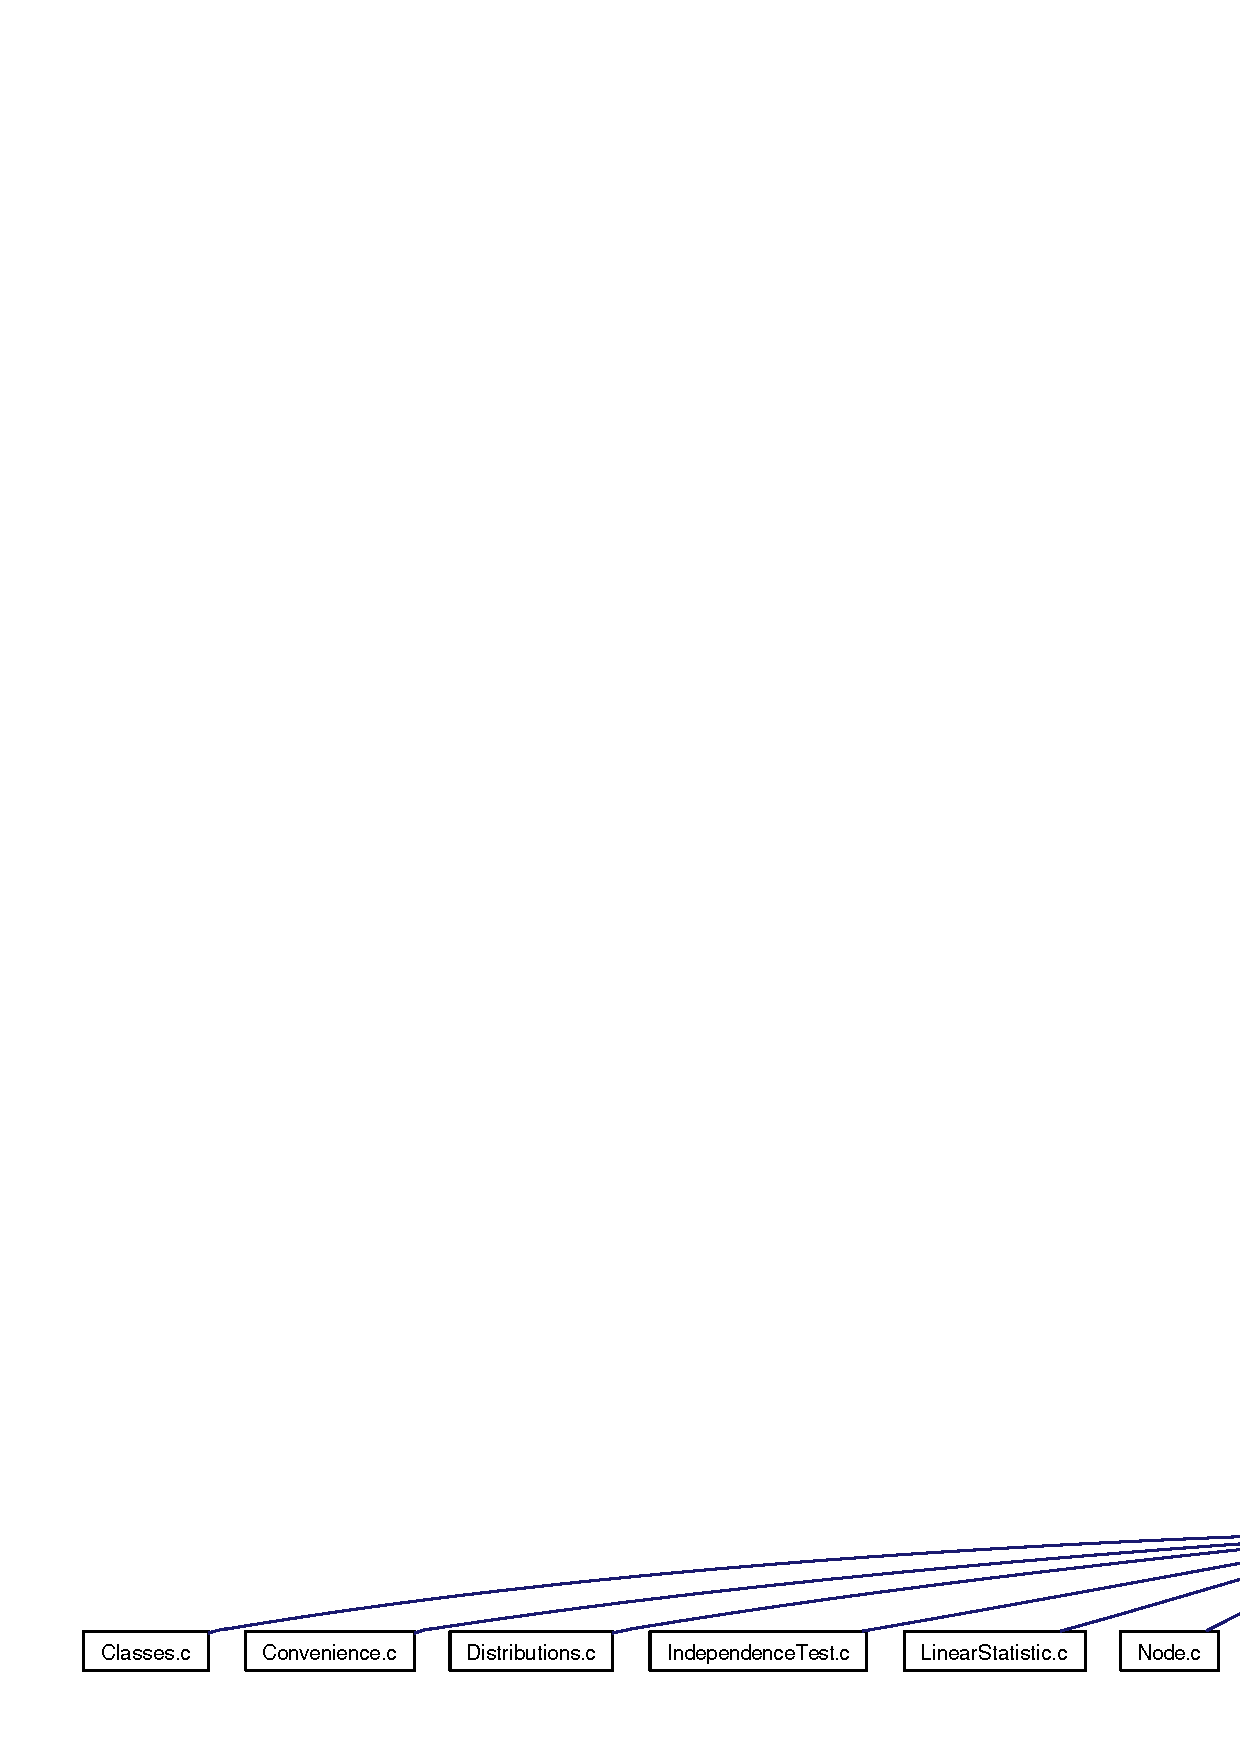
\includegraphics[width=159pt]{Predict_8h__dep__incl}
\end{center}
\end{figure}
\subsection*{Functions}
\begin{CompactItemize}
\item 
void \hyperlink{Predict_8h_a0}{C\_\-splitnode} (SEXP node, SEXP learnsample, SEXP control)
\end{CompactItemize}


\subsection{Function Documentation}
\hypertarget{Predict_8h_a0}{
\index{Predict.h@{Predict.h}!C_splitnode@{C\_\-splitnode}}
\index{C_splitnode@{C\_\-splitnode}!Predict.h@{Predict.h}}
\subsubsection[C\_\-splitnode]{\setlength{\rightskip}{0pt plus 5cm}void C\_\-splitnode (SEXP {\em node}, SEXP {\em learnsample}, SEXP {\em control})}}
\label{Predict_8h_a0}


Split a node according to a splitting rule \par
 \begin{Desc}
\item[Parameters:]
\begin{description}
\item[{\em node}]the current node with primary split specified \item[{\em learnsample}]learning sample \item[{\em control}]an object of class `Tree\-Control' \end{description}
\end{Desc}
\begin{Desc}
\item[\hyperlink{todo__todo000001}{Todo}]outplace the splitting since there are at least 3 functions with nearly identical code \end{Desc}


Definition at line 21 of file Predict.c.

References C\_\-init\_\-node(), get\_\-maxsurrogate(), get\_\-missings(), get\_\-ninputs(), get\_\-nobs(), get\_\-splitctrl(), get\_\-variable(), has\_\-missings(), i\_\-in\_\-set(), ncol(), NODE\_\-LENGTH, PL2\_\-inputs\-Sym, PL2\_\-jointtransf\-Sym, PL2\_\-responses\-Sym, S3\_\-LEFT, S3\_\-RIGHT, S3get\_\-nodeweights(), S3get\_\-primarysplit(), S3get\_\-splitpoint(), S3get\_\-variable\-ID(), and S3is\_\-ordered().

Referenced by C\_\-Tree\-Grow().

Here is the call graph for this function:\begin{figure}[H]
\begin{center}
\leavevmode
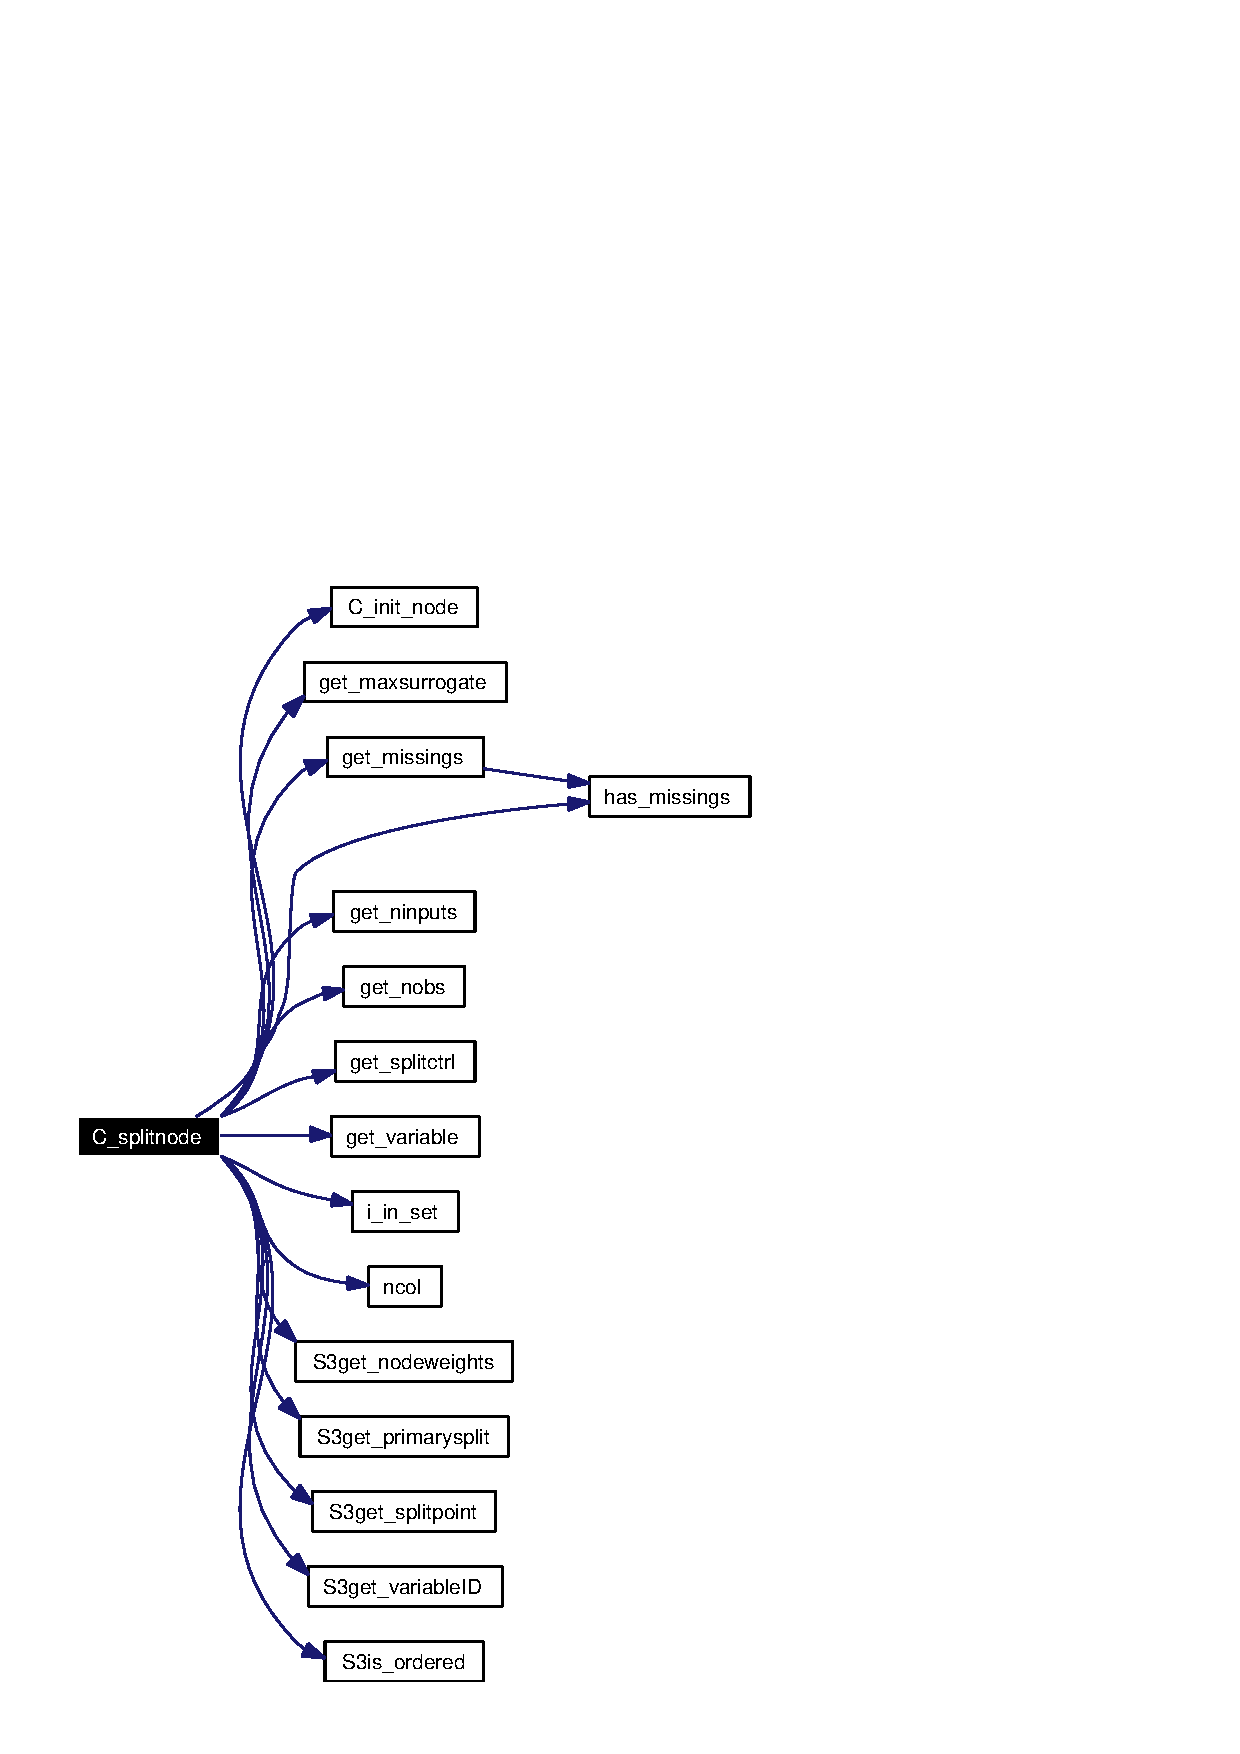
\includegraphics[width=182pt]{Predict_8h_a0_cgraph}
\end{center}
\end{figure}
